\documentclass[
Karos,
%Loesung,
%Punkte
]{pruefung}

\usepackage{pgfplots}

\renewcommand{\Pruefungsfach}{\textbf{Prüfungsfach: Mathematik 2}}
\renewcommand{\Semester}{\textbf{Sommersemester 24}}
\renewcommand{\Studiengaenge}{\textbf{Studiengang: WKB}}
\renewcommand{\Fachnummern}{\textbf{Prüfungsnummer: R39.04355}}
\renewcommand{\Dauer}{\textbf{Zeit: 90 Minuten}}
\renewcommand{\Dozenten}{\textbf{Dozent: Karsten Runge}}

\renewcommand{\Hilfsmittel}{
\textbf{Manuskript\newline
 Literatur \newline
 Taschenrechner Casio FX-87DE Plus / Casio FX-87DE Plus 2nd edition}
}
\renewcommand{\Hinweise}{
\textbf{Bearbeiten Sie die Aufgaben ausschließlich auf diesen Prüfungsblättern.
\newline
Begründen Sie alle Lösungsschritte.}
}

\begin{document}
\begin{Aufgabe}[8]
Hinweis: Alle Teilaufgaben können unabhängig voneinander bearbeitet werden.

\begin{enumerate}
	\item
		Geben Sie eine lineare Differenzialgleichung an, die die Fundamentallösung
		\[
			y(x) = \e^{-2 \, x}
		\]
		besitzt.
		
		\Loesung{80mm}{
		Eigenwert $\lambda_1 = -2$:\hfill\Punkte{2 P}
		\[
			y'(x) = -2 \ y(x) 
		\]
		}
	\item
		Bei welchen Störfunktionen $r$ tritt bei der Differenzialgleichung
		\[
			y'' + 9 \, y = r(x)
		\]
		Resonanz auf?
		Bitte kreuzen Sie den entsprechenden Eintrag an:
		
		\ifLoesung 
		\begin{tabular}{p{0.3\textwidth}p{0.2\textwidth}p{0.2\textwidth}}
			$r(x) = \e^{-9 \, x}$ & $\square$             Resonanz & {\textcolor{red}X} keine Resonanz\\
			$r(x) = \e^{  9 \, x}$ & $\square$             Resonanz & {\textcolor{red}X} keine Resonanz\\
			$r(x) = 3 \, \cos(x)$ & $\square$             Resonanz & {\textcolor{red}X} keine Resonanz\\
			$r(x) = \cos(3 \, x)$ & {\textcolor{red}X} Resonanz &            $\square$  keine Resonanz\\
		\end{tabular}
		\hfill\Punkte{2 P}
		\else
		\begin{tabular}{p{0.3\textwidth}p{0.2\textwidth}p{0.2\textwidth}}
			$r(x) = \e^{-9 \, x}$ & $\square$ Resonanz & $\square$ keine Resonanz\\
			$r(x) = \e^{  9 \, x}$ & $\square$ Resonanz & $\square$ keine Resonanz\\
			$r(x) = 3 \, \cos(x)$ & $\square$ Resonanz & $\square$ keine Resonanz\\
			$r(x) = \cos(3 \, x)$ & $\square$ Resonanz & $\square$ keine Resonanz\\
		\end{tabular}
		\fi
		
		\newpage
		
		\item
			Die folgenden beiden Abbildungen zeigen den zeitlichen Verlauf der Zustände $z_1(t)$ und $z_2(t)$:
			
			\newcommand{\zeins}[1]{1+exp(-0.5*#1)*cos(deg(3*#1))}
			\newcommand{\zzwei}[1]{-0.5*exp(-0.5*x)*cos(deg(3*x))-3*exp(-0.5*x)*sin(deg(3*x))}
			
			\par
			
			\quad 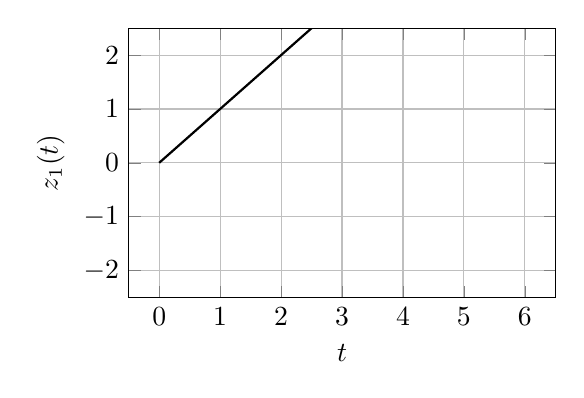
\begin{tikzpicture}
	\begin{axis}[
		xlabel={$t$},
		ylabel={$z_1(t)$},
		xmin=-0.5, xmax=6.5,
		ymin=-2.5, ymax=2.5,
		domain=0:6,
		samples=100,
		grid=major,
		width=7cm,
		height=5cm,
		xtick={0, 1, 2, 3, 4, 5, 6},
		ytick={-2, -1, 0, 1, 2}
		]
		\addplot [
		black,
		thick
		] {\zeins{x}};
	\end{axis}
\end{tikzpicture} \quad \quad \quad 		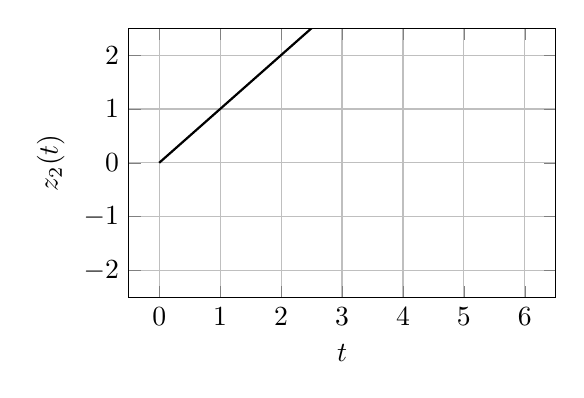
\begin{tikzpicture}
	\begin{axis}[
		xlabel={$t$},
		ylabel={$z_2(t)$},
		xmin=-0.5, xmax=6.5,
		ymin=-2.5, ymax=2.5,
		domain=0:6,
		samples=100,
		grid=major,
		width=7cm,
		height=5cm,
		xtick={0, 1, 2, 3, 4, 5, 6},
		ytick={-2, -1, 0, 1, 2}
		]
		\addplot [
		black,
		thick
		] {\zzwei{x}};
	\end{axis}
\end{tikzpicture}
			
			\par
			
			Welche der folgenden vier Abbildungen zeigt den richtigen Verlauf des Phasenporträts?
			Bitte begründen Sie Ihre Antwort!

			\par

			\quad \input{../M2_IT/m2_it_ss_24_kurzaufgaben_fig3.tex} \hspace*{40mm} 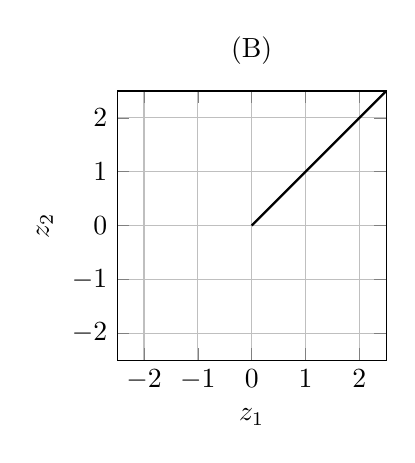
\begin{tikzpicture}
	\begin{axis}[
		title={(B)},
		xlabel={$z_1$},
		ylabel={$z_2$},
		xmin=-2.5, xmax=2.5,
		ymin=-2.5, ymax=2.5,
		domain=0:6,
		samples=100,
		grid=major,
		width=5cm,
		height=5cm,
		xtick={-2, -1, 0, 1, 2},
		ytick={-2, -1, 0, 1, 2}
		]
		\addplot [
		black,
		thick
		] (
		{\zeins{x}}, 
		{\zzwei{x}}
		);
	\end{axis}
\end{tikzpicture}
			
			\par

			\quad 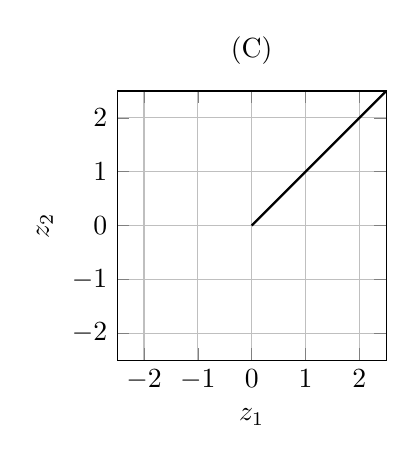
\begin{tikzpicture}
	\begin{axis}[
		title={(C)},
		xlabel={$z_1$},
		ylabel={$z_2$},
		xmin=-2.5, xmax=2.5,
		ymin=-2.5, ymax=2.5,
		grid=major,
		domain=0:6,
		samples=100,
		width=5cm,
		height=5cm,
		xtick={-2, -1, 0, 1, 2},
		ytick={-2, -1, 0, 1, 2}
		]
		\addplot [
		black,
		thick
		] (
		{\zzwei{x}},
		{\zeins{x}}
		);
	\end{axis}
\end{tikzpicture} \hspace*{40mm} \input{../M2_IT/m2_it_ss_24_kurzaufgaben_fig6.tex}

	\Loesung{}{
		Die Spirale endet in der Nähe des Punktes mit den Koordinaten $(1 \mid 0)$.
		Die Werte des Zustands $z_1$ bewegen sich zwischen $0$ und $2$.
		Somit zeigt Abbildung (B) den richtigen Verlauf.
		\hfill\Punkte{2 P}
	}
		
	\newpage
	
		\item
			Beurteilen Sie den folgenden Dialog mit ChatGPT 3.5.
			Sind die Berechnungen und die Behauptungen von ChatGPT korrekt?
			Es genügt den Fehler zu finden, die richtige Lösung muss nicht bestimmt werden!
		
			\textbf{You:} Wie lautet die Lösung des Anfangswertproblems (AWP)
			\[
				x' \cdot x = t, \quad x(0) = 1 \, ?
			\]
		
			\textbf{ChatGPT 3.5:} Um das AWP zu lösen, können wir das Verfahren der Trennung der Variablen verwenden.
		
			1. Trenne die Variablen:
			\[ \frac{{dx}}{{x}} = t \, dt \]
			2. Integriere beide Seiten:
			\[ \int \frac{{dx}}{{x}} = \int t \, dt \quad \Longleftrightarrow \quad \ln|x| = \frac{{t^2}}{2} + C \]
			3. Löse nach \(x\) auf:
			\[ |x| = e^{\frac{{t^2}}{2} + C} \]
			Da \(x(0) = 1\), setzen wir \(t = 0\) und lösen für \(C\):
			\[ |1| = e^C \quad \Longleftrightarrow \quad C = 0 \]
			4. Setze \(C\) ein und berücksichtige das Betragszeichen:
			\[ |x| = e^{\frac{{t^2}}{2}} \quad \Longleftrightarrow \quad  x = \pm e^{\frac{{t^2}}{2}} \]
			Da \(x(0) = 1\), wählen wir das positive Vorzeichen:
			\[ x(t) = e^{\frac{{t^2}}{2}} \]
			
		\Loesung{}{
			Die Trennung der Variablen ist falsch, richtig ist:
			\hfill{\Punkte{2 P}}
			\[ x \cdot \frac{dx}{dt} = t \quad \Longleftrightarrow \quad \int x \, dx = \int t \, dt \]
			Hinweis: ChatGPT 4.0 bestimmt die Lösung des AWP korrekt!
		}
\end{enumerate}
\end{Aufgabe}

\newpage

\endinput
\begin{Aufgabe}[10]% vgl. SS 18
	Wir betrachten das Anfangswertproblem
	\[
		y'(x) \cdot y(x) = \sin(x), \quad y(0) = -1 \, .
	\]
	\begin{enumerate}
		\item
			Handelt es sich um eine lineare oder um eine nichtlineare Differenzialgleichung?
		\item
			Bestimmen Sie die exakte Lösung des Anfangswertproblems.
		\item
			Berechnen Sie einen Näherungswert für $y(1)$, indem Sie mit der Schrittweite $h=\displaystyle\frac{1}{2}$ zwei Schritte mit dem Polygonzugverfahren von Euler durchführen.
		\item
			Wie groß ist die Abweichung des in Aufgabenteil \textbf{c)} berechneten Näherungswerts von der exakten Lösung?
	\end{enumerate}
	
	\Loesung{}{
		\begin{enumerate}[series=dgl_erster_ordnung]
			\item
			Nichtlineare Differenzialgleichung.
			\hfill\Punkte{1 P}
			\item		
			Separation:
			\hfill\Punkte{1 P}
			\[
				\frac{\mbox{d} \, y}{\mbox{d} \, x} \cdot y = \sin(x)
				\quad \Longrightarrow \quad
				\int y \, \mbox{d} \, y = \int \sin(x) \, \mbox{d} \, x
			\]
			Integration:
			\hfill\Punkte{1 P}
			\[
				\frac{1}{2} \, y^2 = -\cos(x) + C
			\]
			Allgemeine Lösung:
			\hfill\Punkte{1 P}
			\[
				y(x) = \pm \sqrt{2 \, C - 2 \, \cos(x)}
			\]
			Anfangswert $y(0) = -1$:
			\hfill\Punkte{1 P}
			\[
				\frac{1}{2} \cdot (-1)^2 = -\cos(0) + C
				\quad \Longrightarrow \quad
				C = \frac{3}{2}
			\]
			Lösung des Anfangswertproblems:
			\hfill\Punkte{1 P}
			\[
				y(x) = -\sqrt{3 - 2 \, \cos(x)}
			\]
			\item
			1. Schritt mit $x_0=0$ und $y_0 = -1$:
			\hfill\Punkte{1 P}
			\[
				y_1 = y_0 + h \, \frac{\sin(x_0)}{y_0} = -1, \quad x_1 = x_0 + h = \frac{1}{2}
			\]
			2. Schritt:
			\hfill\Punkte{1 P}
			\[
				y_2 = y_1 + h \, \frac{\sin(x_1)}{y_1} = -1 - \frac{1}{2} \sin\left( \frac{1}{2} \right) \approx -1.2397,  \quad x_2 = x_1 + h = 1
			\]
		\end{enumerate}
	}
	
	\newpage
	
	\Loesung{}{
		\begin{enumerate}[resume=dgl_erster_ordnung]
			\item
			Exakte Lösung:
			\hfill\Punkte{1 P}
			\[
				y(1) = -\sqrt{3 - 2 \, \cos(1)} \approx - 1.3854
			\]
			Abweichung:
			\hfill\Punkte{1 P}
			\[
				\left| y(1) - y_2 \right| \approx \left| - 1.3854 + 1.2397 \right| \approx 0.1457
			\]
		\end{enumerate}	
		}
\end{Aufgabe}

\newpage

\endinput
\begin{Aufgabe}[9]% vgl. WS 18/19
	Ein Differenzialgleichungssystem ist gegeben durch
	\[
	\begin{array}{ccrcr}
		\dot{x} & = &  -2 \, x & + & 3 \, y \\
		\dot{y} & = &  10 \, x & - & 3 \, y  \\
	\end{array}
	\]
	\begin{enumerate}
		\item
			Bestimmen Sie die allgemeine Lösung des Differenzialgleichungssystems.
		\item
			Ist das System asymptotisch stabil?
	\end{enumerate}
	%
	% Lösung
	%
	\Loesung{}{
		\begin{enumerate}
		\item
		Homogenes System in Matrixform:
		\[
		\left(
		\begin{array}{c}
			\dot{x}\\
			\dot{y}
		\end{array}
		\right)
		=
		\left(
		\begin{array}{rr}
			-2 &  3\\
			10 & -3
		\end{array}
		\right)
		\left(
		\begin{array}{c}
			x\\
			y
		\end{array}
		\right)
		\hfill \Punkte{1 P}
		\]
		Charakteristische Gleichung und Eigenwerte:
		\[
		\left|
		\begin{array}{cc}
			-2 -\lambda &  3\\
			10 & -3 -\lambda
		\end{array}
		\right|
		= \lambda^2 + 5\lambda - 24 = 0
		\quad \Longrightarrow \quad
		\lambda_1 = -8, \, \lambda_2=3
		\hfill \Punkte{2 P}
		\]
		Berechnung eines Eigenvektors
		$\begin{pmatrix}
			u_1\\
			v_1
		\end{pmatrix}$
		zum Eigenwert $\lambda_1=-8$:
		\[
		\begin{pmatrix}
			6 & 3\\
			10 & 5
		\end{pmatrix}
		\begin{pmatrix}
			u_1 \\
			v_1
		\end{pmatrix}
		=
		\begin{pmatrix}
			0\\
			0
		\end{pmatrix}
		\quad \Longrightarrow \quad
		v_1 = -2 \, u_1
		\quad \Longrightarrow \quad 
		\begin{pmatrix}
			u_1\\
			v_1
		\end{pmatrix}
		=
		\begin{pmatrix}
			1\\
			-2
		\end{pmatrix}
		\hfill \Punkte{2 P}
		\] 
		Berechnung eines Eigenvektors
		$\begin{pmatrix}
			u_2\\
			v_2
		\end{pmatrix}$
		zum Eigenwert $\lambda_2=3$: 
		\[
		\begin{pmatrix}
			-5 &  3\\
			10 & -6
		\end{pmatrix}
		\begin{pmatrix}
			u_2\\
			v_2
		\end{pmatrix}
		=
		\begin{pmatrix}
			0\\
			0
		\end{pmatrix}
		\quad \Longrightarrow \quad
		5 \, u_2 = 3 \, v_2
		\quad \Longrightarrow \quad
		\begin{pmatrix}
			u_2\\
			v_2
		\end{pmatrix}
		=
		\begin{pmatrix}
			3\\
			5
		\end{pmatrix}
		\hfill \Punkte{2 P}
		\]
		Allgemeine Lösung des homogenen Differenzialgleichungssytems:
		\[
		\begin{pmatrix}
			x(t)\\
			y(t)
		\end{pmatrix}
		= C_1 \, \mbox{e}^{-8 \, t}
		\begin{pmatrix}
			1\\
			-2
		\end{pmatrix}
		+ C_2 \, \mbox{e}^{3 \, t}
		\begin{pmatrix}
			3\\
			5
		\end{pmatrix}
		\hfill \Punkte{1 P}
		\]
		\item
			Das System ist nicht asymptotisch stabil, da nicht alle Eigenwerte $\lambda$ die Bedingung $\mbox{Re}(\lambda)<0$ erfüllen, $\mbox{Re}(\lambda_2) = 3 > 0$.
			\hfill \Punkte{1 P}
		\end{enumerate}
	}
	
	\newpage
	
	\ifLoesung
	\else
	\Loesung{}{}
	\fi
	
\end{Aufgabe}

\newpage

\endinput
%
% Differenzengleichung ähnlich zu WS 23/24, da Ergebnisse der Studierenden im WS 23/24 nicht gut waren!
% 
\begin{Aufgabe}[10] 
	Eine Differenzengleichung erster Ordnung ist gegeben durch
	\[
		20 \, x_{k+1} - 21 \, x_k = -200, \quad x_0 = 100, \quad k = 0,1,2,3,\ldots . 
	\]
	\begin{enumerate}
		\item
			Geben Sie die Zahlenwerte von $x_1$ und $x_2$ an.
		\item
			Bestimmen Sie die Lösung der Differenzengleichung.
		\item
			Interpretieren Sie die Zahlenfolge $(x_k)$ als Kontostand nach $k$ Jahren, eines Kontos mit festem Zinsatz von dem am Ende jeden Jahres der selbe Betrag abgehoben wird.
			Wie hoch sind Zinsatz und Betrag?
			Wie oft kann der Betrag von dem Konto abgehoben werden bevor der Kontostand negativ wird?
	\end{enumerate}
	
	\Loesung{}{
		\begin{enumerate}[series=differenzengleichung]
			\item
				Rekursionsformel auflösen:
				\hfill\Punkte{1 P}
				\[
					x_{k+1} = \frac{21}{20} \, x_k - 10 \, .
				\]
				Zahlenwerte:
				\hfill\Punkte{1 P}
				\begin{flalign*}
					& k = 0: \, x_1 = \frac{21}{20}\, x_0 - 10  = \frac{21}{20} \cdot 100 - 10 = 95 \, .\\
					& k = 1:  \, x_2 = \frac{21}{20}\, x_1 - 10  = \frac{21}{20} \cdot  95 - 10 = 89.75 \, .
				\end{flalign*}
			\item
				Homogene Lösung:
				\hfill\Punkte{1 P}
				\[
					20 \, x_{k+1} - 21 \, x_k = 0,
					\quad \Longrightarrow \quad
					20 \, \lambda - 21 = 0
					\quad \Longrightarrow \quad
					\lambda = \frac{21}{20}
					\quad \Longrightarrow \quad
					x_k^h = C \cdot \left( \frac{21}{20} \right)^k \, .
				\]
				Partikuläre Lösung:
				\hfill\Punkte{1 P}
				\[
					x_k^p = A
					\quad \Longrightarrow \quad
					20 \, A - 21 \, A = - 200
					\quad \Longrightarrow \quad
					A = 200 \, .
				\]
				Allgemeine Lösung:
				\hfill\Punkte{1 P}
				\[
					x_k = x_k^h + x_k^p = C \cdot \left( \frac{21}{20} \right)^k + 200 \, .
				\]
				Anfangswert $x_0 = 100$: 
				\hfill\Punkte{1 P}
				\[
					k = 0: \quad 
					x_0 = C \cdot \left( \frac{21}{20} \right)^0 + 200
					\quad \Longrightarrow \quad
					100 = C + 200
					\quad \Longrightarrow \quad
					C = -100 \, .
				\]
				Ergebnis:
				\hfill\Punkte{1 P}
				\[
					x_k = -100 \cdot \left( \frac{21}{20} \right)^k + 200 \, .
				\]
		\end{enumerate}
	}
	
	\newpage
	
	\Loesung{}{
		\begin{enumerate}[resume=differenzengleichung]
			\item
				Zinssatz $\frac{21}{20} - 1 = \frac{1}{20} = 5 \%$, Betrag $10$.
				\hfill\Punkte{1 P}
				\par
				Bedingung $x_k = 0$:
				\hfill\Punkte{1 P}
				\[
					100 \cdot \left( \frac{21}{20} \right)^k = 200
					\quad \Longleftrightarrow \quad
					\left( \frac{21}{20} \right)^k  = 2
				\]
				Nach $k$ auflösen:
				\hfill\Punkte{1 P}
				\[
					\ln(2) = \ln\left( \frac{21}{20} \right)^k
					\quad \Longleftrightarrow \quad
					\ln(2) = k \, \ln\left( \frac{21}{20} \right)
					\quad \Longleftrightarrow \quad
					k = \frac{\ln(2)}{ \ln\left( \frac{21}{20} \right)} \approx 14.2
				\]
				Der Betrag kann $14$ mal abgehoben werden. 
		\end{enumerate}
		\par
		\vspace*{10mm}
		\par
		Alternative Lösung für \textbf{b)} mit Lösungsformel für lineare Differenzengleichung erster Ordnung:
		\[
			x_{k+1} = \lambda \, x_k + r_k
			\quad \Longrightarrow \quad
			x_k = \lambda^k \cdot x_0 + \sum_{l=0}^{k-1} \lambda^{k-1-l} r_l \, .
		\]
		Mit $\lambda = \frac{21}{20}$, $r_k = -10$, $x_0 = 100$:
		\[
			x_k =  \left( \frac{21}{20} \right)^k \cdot 100 + \sum_{l=0}^{k-1}\left( \frac{21}{20} \right)^{k-1-l} \cdot (-10) \, .
		\]
		Geometrische Reihe:
		\[
			\sum_{l=0}^{k-1}q^{k-1-l}  = \frac{1- q^k}{1 - q}\, .
		\]
		Mit $q = \frac{21}{20} $:
		\[
			x_k
			= 100 \, \left( \frac{21}{20} \right)^k - 10 \, \frac{1 - \left( \frac{21}{20} \right)^k}{1 - \frac{21}{20}} 
			= 100 \, \left( \frac{21}{20} \right)^k + 200 \, \left(1 - \left( \frac{21}{20} \right)^k \right)
			= -100 \cdot \left( \frac{21}{20} \right)^k + 200 \, .
		\]
	}
	
\end{Aufgabe} 

\newpage

\endinput
\begin{Aufgabe}[8] 
Insa möchte ihrem Bruder Till \textbf{5000 Euro} leihen, die ihm noch fehlen, um ein Auto finanzieren zu können. In dieser Aufgabe werde mit einem Zinssatz von \textbf{2\% p.a.} gerechnet.
\begin{enumerate}
	\item 
	Insa möchte, dass ihr Bruder in \textbf{5 jährlichen Raten} von jeweils \textbf{1000 Euro} den Kredit zurückzahlt. Dabei soll nach einem Jahr die erste Rate gezahlt werden.
	Welchen Verlust macht Insa bei dieser Rückzahlunsvariante, wenn als Zeitpunkt für die Berechnung die Auszahlung der 5000 Euro an Till genommen wird?
	\item 
	Durch welche jährliche Rate E müssten die 1000 Euro in Aufgabe a) ersetzt werden, damit Insa keinen Verlust macht?
	\item
	Till ist seiner Schwester besonders dankbar und macht daher folgenden Vorschlag: Er könnte unbegrenzt jedes Jahr eine Rate von \textbf{400 Euro} zahlen ohne jemals die Zahlungen einzustellen. Auch bei dieser Variante werde die erste Rate nach einem Jahr bezahlt. Welchen Barwert hätte diese Zahlungsfolge, wenn man annimmt, dass die Zahlungen tatsächlich niemals aufhören? 
	
\end{enumerate}

\Loesung{}{
\begin{enumerate}
	\item Der Barwert der Zahlungsfolge liegt bei 
	\hfill\Punkte{2 P}
	\[B=\frac{1000}{1.02}+\frac{1000}{1.02^2}+\frac{1000}{1.02^3}+\frac{1000}{1.02^4}+\frac{1000}{1.02^5}=1000\cdot \frac{1.02^5-1}{1.02^5\cdot (1.02-1)}\approx4713.46\;\text{(Euro)}\]
	Insas Verlust bezogen auf den Auszahlungszeitpunkt beträgt damit 
	\hfill\Punkte{1 P}
	\[5000-4713,46=286.54 \;\text{(Euro)}\]
	\item 
	Setze
	\hfill\Punkte{2 P}
	\[5000=E\cdot \frac{1.02^5-1}{1.02^5\cdot (1.02-1)}\]
	Umstellen nach E ergibt
	\[E=5000\cdot \frac{1.02^5\cdot (1.02-1)}{1.02^5-1}\approx1060.79 \; \text{(Euro)}\]
	\item 
	Für den Barwert B der unendlichen Zahlungsfolge ergibt sich mit der geometrischen Reihe 
	\hfill\Punkte{3 P}
	\[B=400\cdot(\frac{1}{1.02}+\frac{1}{1.02^2}+\frac{1}{1.02^3}+...)=400\cdot\frac{1}{1.02}\cdot \frac{1}{1-\frac{1}{1.02}}=400\cdot \frac{1}{1.02}\cdot \frac{1.02}{1.02-1}\]
	und damit 
	\[B=\frac{400}{0.02}=20000 \; \text{(Euro)}\]
\end{enumerate}
}
 \ifLoesung
\else
\newpage
\Loesung{}{}
\fi

\end{Aufgabe}

\newpage


\endinput
\begin{Aufgabe}[9]
	
Gegeben ist das lineare Optimierungsproblem 
\[ 
f(\vec x)=\vec c\cdot \vec x\stackrel{!}{=}\mathrm{Max}, \quad \mathbf A\vec x\leq \vec b,\quad \vec x\geq 0, 
\] 
mit 
\[ 
\vec    c = \left(\begin{array}{c} 2\\ 6 \end{array}\right),\quad 
\mathbf A = \left(\begin{array}{cc} 2 &-2\\ -1 & 2 \end{array}\right),\quad 
\vec    b = \left(\begin{array}{c} 0\\ 4 \end{array}\right)\,. 
\] 
\begin{enumerate} 
	\item Zeichnen Sie den zulässigen Bereich in das gegebene Koordinatensystem ein. 
	\item Zeichnen Sie im zulässigen Bereich alle Punkte $(x_1,x_2)$ mit $f(x_1,x_2)=12$ ein. 
	\item Wenden Sie den Primalen Simplex-Algorithmus auf dieses Optimierungsproblem an. 
	\item Wäre das gegebene Optimierungsproblem für \[\mathbf A = \left(\begin{array}{cc} -2 & 2\\ -1 & 2 \end{array}\right) \quad  \] lösbar? 
	Begründen Sie Ihre Antwort. 
	 
	 
\end{enumerate} 
	
	\begin{center}  
		\begin{tikzpicture}[xscale=1,yscale=1]  
			\draw[help lines,step=0.5] (-2.5,-5.0) grid (15.0,8.5);  
			\draw[->, darkgray, line width=1pt] (-1.5,0) -- (8.0,0) node[below] {$x_1$};  
			\draw[->, darkgray, line width=1pt] (0,-1.5) -- (0,7.0) node[left] {$x_2$};  
			\foreach \i in {-1,...,-1} { \draw (\i,0.1) -- (\i,-0.1) node[below] {$\i$}; }  
			\foreach \i in {1,...,7} { \draw (\i,0.1) -- (\i,-0.1) node[below] {$\i$}; }  
			\foreach \i in {1,...,6} { \draw (0.1,\i) -- (-0.1,\i) node[left] {$\i$}; }  
			\foreach \i in {-1,...,-1} {\draw (0.1,\i) -- (-0.1,\i) node[left] {$\i$};}  
			\ifLoesung  
			\coordinate[] (P) at (0,2); \fill (P) circle (2pt);  
			% \coordinate[label=] (Q) at (0,2); \fill (Q) circle (2pt);  
			\coordinate[label=] (R) at (0,0); \fill (R) circle (2pt);  
			% \coordinate[label= ] (S) at (2,4); \fill (S) circle (2pt);  
			\coordinate[label= ] (T) at (4,4); \fill (T) circle (2pt);  
			
			% Dreieck zeichnen -------------------------------------------------
			\draw[fill=black!25,thick] 
			(0,2) node (A) [label=right:$$] {} --
			(4,4) node (B) [label=above:$$] {} --
			(0,0) node (C) [label=above left:$$] {} -- 
			cycle;
			% ------------------------------------------------------------------
			\coordinate[label= right: Zulässigkeitsbereich  ] (S1) at (0.75,2.75);   
			\coordinate[label= right: Isolinie ] (S2) at (1.5,1.25);  
			
			%\draw[ultra thick,-] (2,0)--(4,4);  
			% \draw[ultra thick,-] (2,4)--(4,2);  
			%\draw[ultra thick,-] (0,0)--(4,4); 
			% \draw[ultra thick,-] (0,0)--(2,0);  
			%\draw[ultra thick,-] (0,0)--(0,2);  
			\draw[gray, dashed, ultra thick,-] (0, 2)--(1.5, 1.5);  
			\fi  
		\end{tikzpicture}  
	\end{center}  
	\clearpage 
	
	
	\Loesung{}{
		
	\begin{enumerate} 
		\item Zulässigkeitsbereich: siehe Skizze.     \hfill\Punkte{2} 
		\item Isolinie $f(x_1,x_2)=6$: siehe Skizze.  \hfill\Punkte{1} 
		\item Das LOP ist in Standardformat gegeben, d.h. eine zulässige Basislösung existiert. \\ 
		Das Ausgangstableau lautet 
		\[ 
		\begin{array}{c|cc|cc|c} 
			\mbox{BV} &  x_1 & x_2 & z_1 & z_2 & b_i  \\ \hline 
			z_1      & 2 & -2 & 1 & 0 & 0  \\ 
			z_2      & -1 & 2 & 0 & 1 & 4  \\ \hline 
			f        & 2 & 6 & 0 & 0 & 0  \\ 
		\end{array} 
		\hfill\Punkte{1} 
		\] 
		$1$. Schritt: 
		Pivot-Spalte: $2$; Pivot-Zeile: $2$. Die Nichbasisvariable $x_{2}$ wird in die Basis aufgenommen. Dies führt auf das Tableau 
		\[ 
		\begin{array}{c|cc|cc|c} 
			\mbox{BV}   &  x_1                    & x_2                     & z_1                     & z_2                     & b_i  \\ \hline 
			z_1 & 1 & 0 & 1 & 1 & 4 \\ 
			x_{2}  & -\frac{1}{2} & 1 & 0 & \frac{1}{2} & 2 \\ \hline 
			f          & 5 & 0 & 0 & -3 & -12 \\ 
		\end{array} 
		\hfill\Punkte{2} 
		\] 
		$2$. Schritt: 
		Pivot-Spalte: $1$; Pivot-Zeile: $1$. Die Nichbasisvariable $x_{1}$ wird in die Basis aufgenommen. Dies führt auf das Tableau 
		\[ 
		\begin{array}{c|cc|cc|c} 
			\mbox{BV}   &  x_1                    & x_2                     & z_1                     & z_2                     & b_i  \\ \hline 
			x_{1}  & 1 & 0 & 1 & 1 & 4 \\ 
			x_{2}  & 0 & 1 & \frac{1}{2} & 1 & 4 \\ \hline 
			f          & 0 & 0 & -5 & -8 & -32 \\ 
		\end{array} 
		\hfill\Punkte{2} 
		\] 
		Die Zielfunktionszeile enthält nur Elemente $\leq 0$. Dies entspricht der 1. Abbruchbedingung. \\ Die optimale zulässige Lösung ist $(x_1,x_2)=(4,4)$ mit $f(x_1,x_2)= 32$. \\ 
		 
		\item Nein, denn der Zulässigkeitsbereich wäre unbeschränkt. \hfill\Punkte{1} 
	\end{enumerate} 	
	}
	
	\ifLoesung
	\else
	\newpage
	\Loesung{}{}
	\fi
	
\end{Aufgabe}

\newpage

\endinput
\end{document}
